\documentclass{article}
%\usepackage[spanish,activeacute]{babel}
%\usepackage[english,activeacute]{babel}
%\usepackage[latin1]{inputenc}
\usepackage[utf8]{inputenc}
\usepackage[english]{babel}
\usepackage{amsmath,amsfonts,amssymb,amstext,amsthm,amscd}
\usepackage{hyperref}
\usepackage{latexsym}
\usepackage{graphicx}
%\usepackage{subfigure}
\usepackage{subfig}
%\linespread{1.6}
\usepackage{float}
\usepackage{dcolumn}% Align table columns on decimal point(esto lo saque del ejemplo de revtex4)
\usepackage{bm}% bold math(esto lo saque del ejemplo de revtex4)
\newcounter{itemR}
\usepackage{here} \usepackage{fancyhdr}
%\usepackage{sidecap}
%\usepackage[spanish,activeacute]{babel}
\usepackage{multirow}
\usepackage{multicol}
\usepackage{array}
\usepackage{ragged2e}
%\usepackage{booktabs}% para hacer tablas profesionales con \toprule

% ------------------------------------------------------------------------------------------------------------------------------------------------------

\usepackage{fancyhdr}
\setlength{\headheight}{15.2pt}
\usepackage[paperwidth=8.5in, paperheight=11.0in, top=1.0in, bottom=1.0in, left=1.0in, right=1.0in]{geometry}

\pagestyle{fancyplain}
\fancyhead[LE,RO]{Reporte $\#$6}
\fancyhead[CE,CO]{}
\fancyhead[RE,LO]{P23-LRT2022-3}
\fancyfoot[LE,RO]{\thepage}
\fancyfoot[CE,CO]{Diseño digital, UDLAP}
\fancyfoot[RE,LO]{}

% ------------------------------------------------------------------------------------------------------------------------------------------------------
% ------------------------------------------------------------------------------------------------------------------------------------------------------
% ------------------------------------------------------------------------------------------------------------------------------------------------------

\begin{document}

\fancypagestyle{plain}{
   	\renewcommand{\headrulewidth}{1pt}
   	\renewcommand{\footrulewidth}{1pt}
}

\renewcommand{\footrulewidth}{1pt}
\renewcommand{\tablename}{Tabla}
\renewcommand{\figurename}{Figura}

% ------------------------------------------------------------------------------------------------------------------------------------------------------
% ------------------------------------------------------------------------------------------------------------------------------------------------------
% ------------------------------------------------------------------------------------------------------------------------------------------------------

\title{Circuitos digitales básicos}
\author{\small{Erick Gonzalez Parada ID: 178145 $\&$ Omar Martínez López ID: 177465}\\ 
\small{ Depto. Computación Electrónica y Mecatrónica.} \\
\small {Docente: Dr. Juan Carlos Moreno Rodríguez}}

%\small{Depto. Computación Electrónica y Mecatrónica.}
%\small{Docente: Dr. Juan Carlos Moreno Rodríguez}
     %\small{Docente: Dr. Juan Carlos Moreno Rodríguez}}
\date{\small{\today}}

\maketitle

% ------------------------------------------------------------------------------------------------------------------------------------------------------

\begin{abstract}
	\begin{justify}
		Se programo un display de 7 segmentos en una tarjeta de desarrollo FPGADE10 para que nos mostrase los números decimales siendo los inputs (entradas) los switches que se tienen en la tarjeta de tal manera que representen los numeros binarios y la traducción de estos queden plasmados en el display de 7 segmentos.	
		\end{justify}
{\it Keywords:}   diseño de hardware, display de siete segmentos  
\end{abstract}
\begin{multicols}{2}
\section{Objetivo}\label{Objetivo}
El estudiante desarrolla los circuitos combinacionales necesarios para decodificar un dígito BCD al encendido de un display de 7 segmentos.	
\section{Introducción}\label{sec:intro}
En la actualidad muchos de los aparatos electrónicos con los convivimos día con día funcionan gracias a que en su interior se encuentran las instrucciones de los procesos que estos deben realizar dependiendo de cada dispositivo por su hardware y propósito, y es así que son programados para que cumplan sus funciones. Ejemplo de esto y lo que llevaremos en practica es la implementación de un display de 7 segmentos, todos esto desde el punto más básico buscando las funciones necesarias para cada uno de los números que son mostrados en el display, para después implementarlos en un código para así implementarlo en BCD y así el display puede enseñar el numero deseado.
\begin{figure}[H]
	\centering
	\includegraphics[scale=0.7]{../../static/df1.jpg}	
	\caption{reloj digital}
	\label{fig:1}
\end{figure}
\section{Análisis Teórico}\label{sec:analiTeorico}
los displays de 7 segmentos han estado en la vida cotidiana de muchas personas, desde haciendo relojes digitales, relojes de ajedrez, cronómetros, entre otros.
\begin{figure}[H]
	\centering
	\includegraphics[scale=0.7]{../../static/df2.jpg}	
	\caption{reloj de ajedrez}
	\label{fig:2}
\end{figure}
Es importante mencionar que estas luces no están forzadas a tomar la forma de un número, el diseño de hardware nos permite darle muchas más funcionalidades como por ejemplo mostrar diferentes símbolos que nos ayuden a representar algo.
\section{Procedimiento}\label{sec:procedim}
Primero debemos de tener nuestro programa en VHDL que nos permita escribir la lógica que nos permita representar los números binarios del 0 a 9 con los switches y estos son tratados entonces como las entradas de nuestro programa (valores booleanos).
\\
\\

Después ya con nuestro código en VHDL, podemos ingresar al programa quartus para hacer la vinculación real entre las entradas y salidas de nuestro programa, las salidas en este caso son todas las funciones booleanas que encienden en el momento adecuado para formar al número decimal, por ultimo especificamos que precisamente queremos que nuestro código ya haga las modificaciones de hardware necesarias para ver resultados plasmados en el display de siete segmentos donde se tendrá que ver correctamente el número.

\section{Resultados esperados}\label{sec:resEsperados}
Los resultados esperados son simples y directos
\begin{table}[H]
	\centering
	\begin{tabular}{|c|c|c|}
		\hline
		Binario & Decimal & res. esperado \\
		\hline
		0001 & 1 & 1 \\
		\hline
		0010 & 2 & 2 \\
		\hline
		0011 & 3 & 3 \\
		\hline
		0100 & 4 & 4 \\
		\hline
		0101 & 5 & 5 \\
		\hline
		0110 & 6 & 6 \\
		\hline
		0111 & 7 & 7 \\
		\hline
		1000 & 8 & 8 \\
		\hline
		1001 & 9 & 9 \\
		\hline
		1010 & 10-15 & "-" Error \\
		\hline
	\end{tabular}
	\caption{tabla de resultados esperados}
	\label{table:1}
\end{table}
Como podemos observar en la tabla \ref{table:1} de resultados esperados, cada representación binaria va con su representación decimal hasta que superamos al nueve donde mostraremos un símbolo que por esta ocasión la tratamos como "error".
\section{Resultados obtenidos}\label{sec:resObtenidos}
Como se podrán observar en las siguientes imágenes la secuencia binaria se encuentra en los switches leídos de forma normal y natural, es decir, no ocupamos lógica inversa y asignamos de manera ordenada las entradas para que se coordinen bien con las salidas 
\begin{figure}[H]
	\centering
	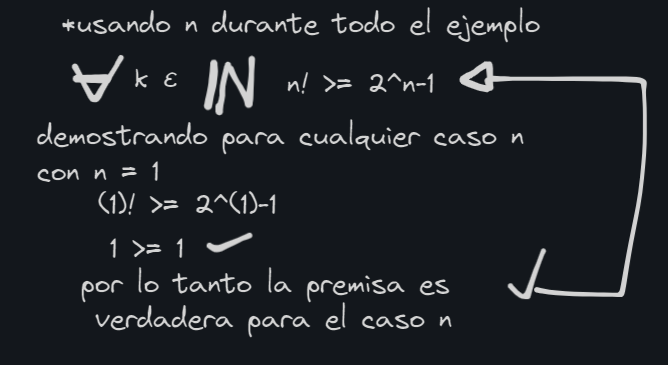
\includegraphics[scale=0.1]{../../static/d0.jpeg}	
	\caption{0}
	\label{fig:3}
\end{figure}

\begin{figure}[H]
	\centering
	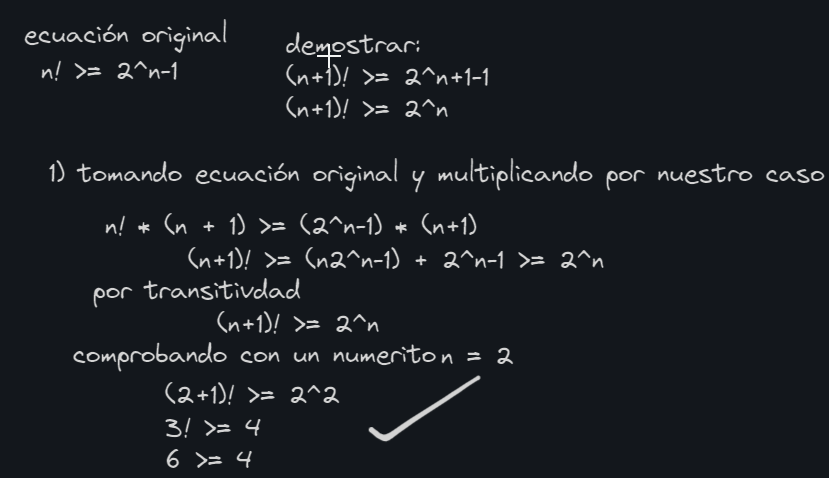
\includegraphics[scale=0.1]{../../static/d1.jpeg}	
	\caption{1}
	\label{fig:4}
\end{figure}

\begin{figure}[H]
	\centering
	\includegraphics[scale=0.1]{../../static/d2.jpeg}	
	\caption{2}
	\label{fig:5}
\end{figure}

\begin{figure}[H]
	\centering
	\includegraphics[scale=0.1]{../../static/d3.jpeg}	
	\caption{3}
	\label{fig:6}
\end{figure}

\begin{figure}[H]
	\centering
	\includegraphics[scale=0.1]{../../static/d4.jpeg}	
	\caption{4}
	\label{fig:7}
\end{figure}

\begin{figure}[H]
	\centering
	\includegraphics[scale=0.1]{../../static/d5.jpeg}	
	\caption{5}
	\label{fig:8}
\end{figure}

\begin{figure}[H]
	\centering
	\includegraphics[scale=0.1]{../../static/d6.jpeg}	
	\caption{6}
	\label{fig:9}
\end{figure}

\begin{figure}[H]
	\centering
	\includegraphics[scale=0.1]{../../static/d7.jpeg}	
	\caption{7}
	\label{fig:10}
\end{figure}

\begin{figure}[H]
	\centering
	\includegraphics[scale=0.1]{../../static/d8.jpeg}	
	\caption{8}
	\label{fig:11}
\end{figure}

\begin{figure}[H]
	\centering
	\includegraphics[scale=0.1]{../../static/d9.jpeg}	
	\caption{9}
	\label{fig:12}
\end{figure}

\begin{figure}[H]
	\centering
	\includegraphics[scale=0.1]{../../static/derror.jpeg}	
	\caption{error}
	\label{fig:13}
\end{figure}




\section{Conclusiones}\label{sec:conclusion}
Como se pudo observar se cumplió el objetivo, los resultados esperados fueron nuestros resultados finales sin mayor complicación. El resultado de esta practica es el reflejo de los aprendizajes aprendidos anteriormente, y ahora son mostrados con unos resultados más fáciles de percibir en nuestro día a día, además de que esto también nos abre las puertas a hacer proyectos mas complejos implementando este display de 7 segmento para mostrar procedimientos o funciones que nos resulten más útiles para implementar en aparatos con funciones específicas.  Por esto es que, aunque parezca un logro sencillo, es algo muy importante que es una base fundamental de dispositivos electrónicos que utilizamos día con día.
\section*{Referencias}\label{sec:referencias}	
No hubo usos de referencias para este trabajo
\end{multicols}
\end{document}

